\documentclass[12pt,letterpaper]{article}
\usepackage[spanish]{babel}
\usepackage[utf8]{inputenc}
\usepackage{graphicx}
\usepackage{pst-pdf}
\usepackage{amssymb}
\usepackage{hyperref}
\usepackage{listings}
\usepackage{biblatex}
\addbibresource{tarea_4.bib} 
\title{{Programacion estructurada.}}
\author{Daniel Reyes Barrera}
\date{19 de noviembre de 2020}

\begin{document}
\maketitle
\abstract{En este documento se ha resuelto algunos problemas computacionales utilizando las herramientas aprendidas de la clase 4 – Programaci\'on estructurada del curso de programaci\'on C++, las cuales son: Estructura de control condicionada (\texttt{if-else} o \texttt{switch-case}), estructuras de control por repetici\'on (\texttt{for}, \texttt{while}, \texttt{do-while}). }


\section{Ejercicio 1.}

Escriba un programa que lea un año y determine si se trata de un año bisiesto.

\subsection{Problema computacional.}
\textbf{Objetivo:} Dado un n\'umero entero como año determinar si es un año bisiesto o no.

\textbf{Entrada:} Un n\'umero entero mayor que 0 representando un año.

\textbf{Salida:} La respuesta de si el n\'umero dado es un año bisiesto o no.

\subsection{Algoritmo.}
Para solucionar el problema computacional, partimos de la definici\'on de un año bisiesto. Un año se denomina bisiesto si es m\'ultiplo de 4, a excepci\'on de que s\'i es m\'ultiplo de 100 tambi\'en y no de 400 entonces no es bisiesto, por tanto necesitaremos utilizar el condicional \texttt{if-else} para validar que se cumplan las condiciones para que el año sea bisiesto o no.


El código fuente está disponible en mi repositorio de git hub. \cite{url:bisiesto}

\subsection{Instancia del problema.}
Como prueba de escritorio, se seleccionaron las siguientes instancias del problema. Entrada: 44, 200, 800 y 122423. La salida del programa se observa en la Figura \ref{fig:bisiesto}.
\begin{figure}[ht!]
  \centering
  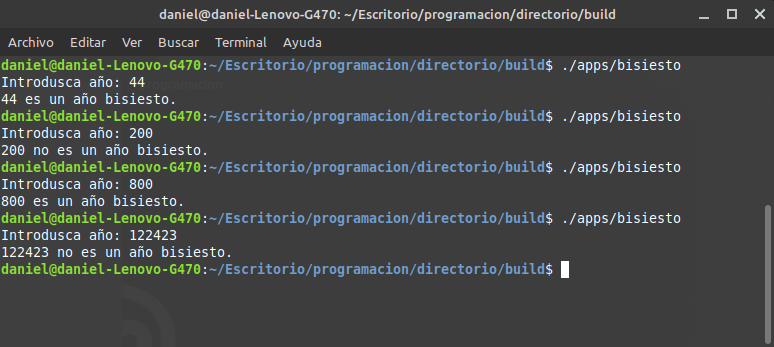
\includegraphics[width=0.8\textwidth]{figures/bisiesto}
  \caption{Ejecución de algunas instancias del problema.}
  \label{fig:bisiesto}
\end{figure}

\section{Ejercicio 2.}

Escriba un programa que capture los coeficientes $a$, $b$, $c$ de un polinomio de segundo orden, e imprima las raices del polinomio.

\subsection{Problema computacional.}
\textbf{Objetivo:} Calcular las raices de un polinomio de segundo orden de manera general.

\textbf{Entrada:} Tres n\'umeros reales que representan los coeficientes del polinomio.

\textbf{Salida:} Las raices (reales o complejas) del polinimio.

\subsection{Algoritmo.}
Para solucionar el problema computacional, sabemos que por la formula general $ x = \frac{-b \pm \sqrt{b^2 - 4ac}}{2a} $ podemos hallar las raices de un polinomio de segundo orden. Si $\sqrt{b^2 - 4ac} \ > \ 0$ entonces el polinomio tiene raices reales, en caso contrario tiene raices complejas.


El código fuente está disponible en mi repositorio de git hub. \cite{url:raices_de_polinomio}

\subsection{Instancia del problema.}
Como prueba de escritorio, se seleccionaron los siguientes polinomios: $  2x^2+6x+3=0$ y $4x^2+2x+5=0$. Donde el primer polinomio tiene raices reales, y el segundo raices complejas. La salida del programa se observa en la Figura \ref{fig:raices_de_polinomio}.
\begin{figure}[ht!]
  \centering
  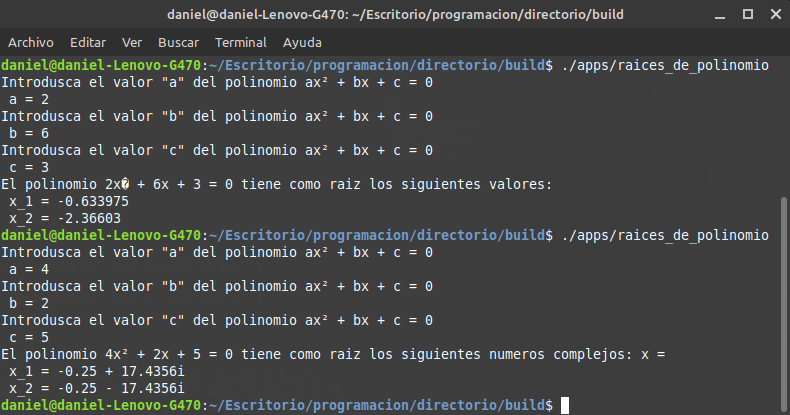
\includegraphics[width=0.8\textwidth]{figures/raices_de_polinomio}
  \caption{Ejecución de algunas instancias del problema.}
  \label{fig:raices_de_polinomio}
\end{figure}

\section{Ejercicio 3.}

Escriba un programa que lea dos n\'umeros y uno de los siguientes operadores: +, -, *, / . El programa debe aplicar y calcular la operaci\'on seleccionada a los n\'umeros introducidos e imprimir el resultado.

\subsection{Problema computacional.}
\textbf{Objetivo:} Dado dos n\'umero y un operador mostrar el resultado de la operaci\'on.

\textbf{Entrada:} Dos n\'umeros reales y un caracter (+ , -, * \'o / ).

\textbf{Salida:} El resultado de la operaci\'on.

\subsection{Algoritmo.}
Para solucionar el problema computacional, se utilizo la estructura de control condicionada \texttt{switch} para realizar la operaci\'on seleccionada.


El código fuente está disponible en mi repositorio de git hub. \cite{url:calcular_operacion}

\subsection{Instancia del problema.}
Como prueba de escritorio, se seleccionaron las siguientes instancias del problema. Entrada: 34, 56, * y 200, 100, -. La salida del programa se observa en la Figura \ref{fig:calcular_operacion}.
\begin{figure}[ht!]
  \centering
  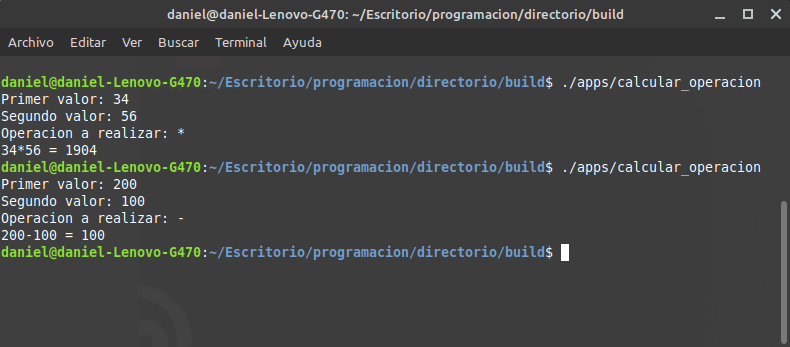
\includegraphics[width=0.8\textwidth]{figures/calcular_operacion}
  \caption{Ejecución de algunas instancias del problema.}
  \label{fig:calcular_operacion}
\end{figure}


\section{Ejercicio 4.}

Escriba un programa que lea una letra y determine si es vocal o consonante. Asuma que el usuario no puede introducir n\'umeros ni caracteres especiales.

\subsection{Problema computacional.}
\textbf{Objetivo:} Dado una letra, determinar si es vocal o consonante.

\textbf{Entrada:} Una letra del abecedario.

\textbf{Salida:} La respuesta de si la letra es una vocal o consonante.

\subsection{Algoritmo.}
Para solucionar el problema computacional, se utilizo el metodo \texttt{toupper()} para tener en cuenta las letras minusculas intruducidas por el usuario, posteriormente se utilizo la estructura de control condicionada \texttt{switch} para validar si la letra introducida por el usuario coincide con una vocal.


El código fuente está disponible en mi repositorio de git hub. \cite{url:vocal_consonante}

\subsection{Instancia del problema.}
Como prueba de escritorio, se seleccionaron las siguientes instancias del problema. Entrada: r, a, Y, O y 4. La salida del programa se observa en la Figura \ref{fig:vocal_consonante}.
\begin{figure}[ht!]
  \centering
  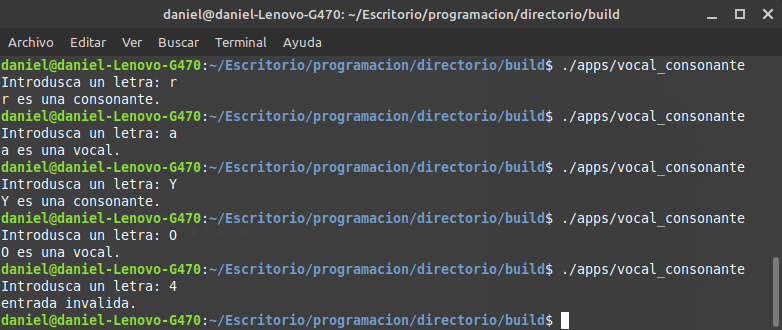
\includegraphics[width=0.8\textwidth]{figures/vocal_consonante}
  \caption{Ejecución de algunas instancias del problema.}
  \label{fig:vocal_consonante}
\end{figure}


\section{Ejercicio 5.}

En el juego para dos personas llamado ''Roca, papel \'o tijera'' cada jugador escoge ''R'', ''P'' o ''T'' respectivamente. El ganador se determina as\'i: roca rompe tijeras, las tijeras cortan el papel, el papel cubre la roca, el juego es un empate si ambos jugadores eligen la misma opci\'on.
Elaborar un programa en que un jugador sea el usuario y el otro la computadora. El programa debe leer la entrada del usuario (R,P, \'o T) y generar la opci\'on elegida por la computadora de forma aleatoria. La salida debe mostrarse de la siguiente forma: ''T-R Roca rompe tijeras: Gana el usuario'' \'o ''P-R Papel cubre roca: Gana la computadora''.

\subsection{Problema computacional.}
\textbf{Objetivo:} Programar el juego de ''Roca, papel \'o tijeras'' donde el usuario juegue contra la computadora.

\textbf{Entrada:} Una letra (R, P \'o T) representando la elecci\'on del usuario.

\textbf{Salida:} El resultado del juego comparando con la elecci\'on de la computadora.

\subsection{Algoritmo.}
Para solucionar el problema computacional, en primer lugar el c\'odigo del juego esta siendo ejecutado en el ciclo \texttt{do-while} preguntandole al usuario si desea segui jugando. Despues utilizamos la libreria \texttt{<ctime>} para tener una semilla diferente \texttt{srand(time(0))} en cada ejecuci\'on del programa y asi obtener valores diferentes en \texttt{rand()} para la elecci\'on de la computadora.


El código fuente está disponible en mi repositorio de git hub. \cite{url:rock_piper}

\subsection{Instancia del problema.}
Como prueba de escritorio, se seleccionaron las siguientes instancias del problema. Primera elecci\'on del usuario: R. Segunda elecci\'on del usuario: t. La salida del programa se observa en la Figura \ref{fig:rock_piper}.
\begin{figure}[ht!]
  \centering
  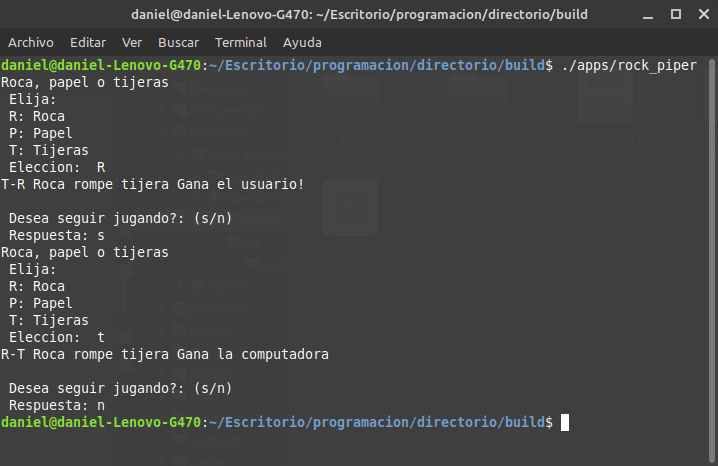
\includegraphics[width=0.8\textwidth]{figures/rock_piper}
  \caption{Ejecución de algunas instancias del problema.}
  \label{fig:rock_piper}
\end{figure}
\newpage

\section{Ejercicio 6.}

Escriba un programa que lea un n\'umero entero $n$, y calcule el resultado de la serie geom\'etrica:
$$ s = \sum_{k=0}^{n-1}\left(\frac{1}{2}\right)^k = 1 + \left(\frac{1}{2}\right)^1 + \left(\frac{1}{2}\right)^2 + \left(\frac{1}{2}\right)^3 + \left(\frac{1}{2}\right)^4 + \left(\frac{1}{2}\right)^5 + ...  + \left(\frac{1}{2}\right)^{n-1} $$

\subsection{Problema computacional.}
\textbf{Objetivo:} Dado un n\'umero entero positivo $n$ calcular el resultado de la serie geom\'etrica hasta el n-simo t\'ermino.

\textbf{Entrada:} Un n\'umero entero positivo n.

\textbf{Salida:} El resultado de la suma hasta el n-simo t\'ermino.

\subsection{Algoritmo.}
Para solucionar el problema computacional, se utilizo la estructura de control por repetici\'on \texttt{for} para ir sumando $n$ veces el resultado de cada termino a una variable de la suma total.


El código fuente está disponible en mi repositorio de git hub. \cite{url:serie_geometrica}

\subsection{Instancia del problema.}
Como prueba de escritorio, se seleccionaron las siguientes instancias del problema. Entradas: $n=3$, $n=7$ y $n=20$ . La salida del programa se observa en la Figura \ref{fig:serie_geometrica}.
\begin{figure}[ht!]
  \centering
  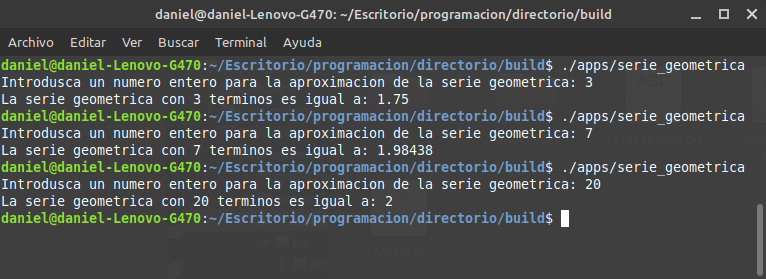
\includegraphics[width=0.8\textwidth]{figures/serie_geometrica}
  \caption{Ejecución de algunas instancias del problema.}
  \label{fig:serie_geometrica}
\end{figure}


\section{Ejercicio 7.}

La sucesi\'on de Fibonacci es un conjunto infinito de n\'umeros ordenados, donde cada elemento de la sucesi\'on es igual a la suma de los dos elementos anteriores. La sucesi\'on comienza con los elementos $0$, $1$ y contin\'ua como se muestra a continuaci\'on: 
$$ 0, 1, 1, 2, 3, 5, 8, 13, 21, 34, 55,... $$
Escriba un programa que imprima los primeros 100 t\'erminos de la serie de
Fibonacci.

\subsection{Problema computacional.}
\textbf{Objetivo:} Calcular los primeros 100 elementos de la serie de fibonnaci.

\textbf{Entrada:} Un n\'umero entero representando la cantidad de t\'erminos deseados.

\textbf{Salida:} Los primeros 100 terminos de la serie de fibonnaci.

\subsection{Algoritmo.}
Para solucionar el problema computacional, se utilizo la estructura de control por repetici\'on \texttt{for} para ir sumando los dos terminos anteriores para hallar el siguiente $n=100$ veces .


El código fuente está disponible en mi repositorio de git hub. \cite{url:fibonnaci}

\subsection{Instancia del problema.}
Como prueba de escritorio, se seleccionó la siguiente instancia del problema. $n=100$ La salida del programa se observa en la Figura \ref{fig:fibonnaci}.
\begin{figure}[ht!]
  \centering
  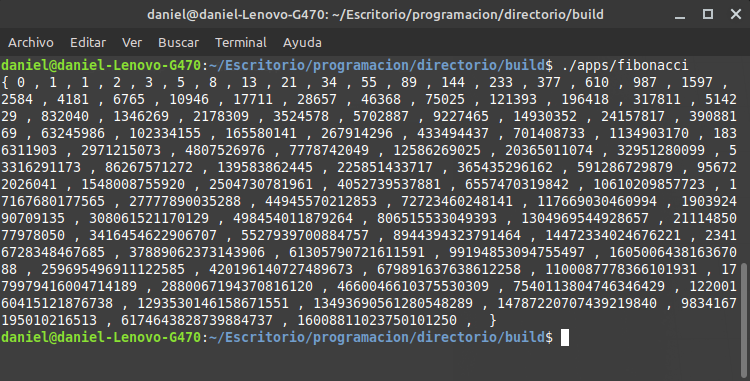
\includegraphics[width=0.8\textwidth]{figures/fibonnaci}
  \caption{Ejecución de algunas instancias del problema.}
  \label{fig:fibonnaci}
\end{figure}


\section{Ejercicio 8.}
\label{ejercicio_8}

En 1682, el matem\'atico alem\'an, Gottfried Leibniz, propuso una f\'ormula para aproximar el valor del n\'umero $\pi$, de la siguiente forma:
$$ \frac{\pi}{4} = \sum_{n=0}^{\infty}\frac{(-1)^n}{2n+1} $$
Esta f\'ormula, es una serie infinita. Sumando un conjunto infinito de t\'erminos, es posible aproximar el valor de $\pi$ con una precisi\'on razonable. Escriba un programa que calcule el valor aproximado de $\pi$. El programa debe preguntar al usuario el n\'umero de t\'erminos con los cuales desea calcular el valor de $\pi$.


\subsection{Problema computacional.}
\textbf{Objetivo:} Dado un n\'umero entero positivo calcular una aproximaci\'on de $\pi$.

\textbf{Entrada:} Un n\'umero entero positivo $n$.

\textbf{Salida:} Una aproximaci\'on de $\pi$ a $n$ t\'erminos.

\subsection{Algoritmo.}
Para solucionar el problema computacional, se despejo el valor de $\pi$ de la ecuaci\'on de Leibniz y utilizo la estructura de control por repetici\'on \texttt{for} para ir sumando $n$ veces los terminos de la ecuaci\'on.

El código fuente está disponible en mi repositorio de git hub. \cite{url:gottried_leibniz}

\subsection{Instancia del problema.}
Como prueba de escritorio, se seleccionaron las siguientes instancias del problema. Entrada: $n=10$, $n=100$, $n=1000$ y $n=10000$. La salida del programa se observa en la Figura \ref{fig:gottried_leibniz}.
\begin{figure}[ht!]
  \centering
  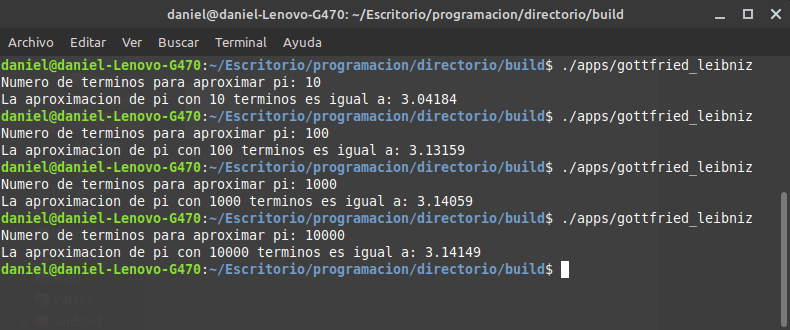
\includegraphics[width=0.8\textwidth]{figures/gottfried_leibniz}
  \caption{Ejecución de algunas instancias del problema.}
  \label{fig:gottried_leibniz}
\end{figure}


\section{Ejercicio 9.}

El problema de Basilea, consiste en calcular la suma exacta de los inversos de los cuadrados de los n\'umeros enteros positivos. En 1735, el matem\'atico suizo Leonhard Euler solucion\'o dicho problema, de tal forma que:
$$ \sum_{n=1}^{\infty}\frac{1}{n^2} = \frac{\pi^2}{6} $$
Escriba un programa que utilizando esta f\'ormula calcule el valor
aproximado de $\pi$. El programa debe preguntar al usuario el n\'umero de t\'erminos con los cuales desea calcular el valor de $\pi$.

\subsection{Problema computacional.}
\textbf{Objetivo:} Dado un n\'umero entero positivo calcular una aproximaci\'on de $\pi$.

\textbf{Entrada:} Un n\'umero entero positivo $n$.

\textbf{Salida:} Una aproximaci\'on de $\pi$ con $n$ t\'erminos.

\subsection{Algoritmo.}

Para solucionar el problema computacional, se hizo un procedimiento similar al ejercicio \ref{ejercicio_8}


El código fuente está disponible en mi repositorio de git hub. \cite{url:basilea}

\subsection{Instancia del problema.}
Como prueba de escritorio, se seleccionaron las siguientes instancias del problema. Entrada: $n=400$, $n=1000$ y $n=10000$. La salida del programa se observa en la Figura \ref{fig:basilea}.
\begin{figure}[ht!]
  \centering
  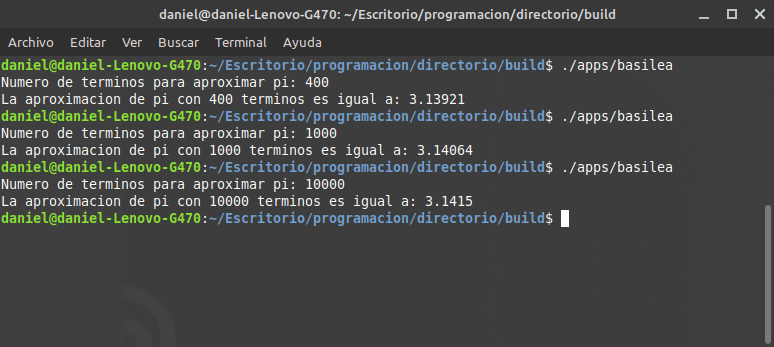
\includegraphics[width=0.8\textwidth]{figures/basilea}
  \caption{Ejecución de algunas instancias del problema.}
  \label{fig:basilea}
\end{figure}


\section{Ejercicio 10.}

La siguiente se llama conjetura de ULAM:
\begin{itemize}
	\item Comience con cualquier n\'umero entero positivo. 
	\item Si es par div\'idalo entre 2, si es impar multipl\'iquelo por 3 y agr\'eguele 1.
	\item Obtenga enteros sucesivamente repitiendo el proceso.
	\item Al final, obtendr\'a el n\'umero 1, independientemente del entero inicial.
\end{itemize}
Escriba un programa que lea un n\'umero entero positivo y obtenga e imprima la sucesi\'on de ULAM.

\subsection{Problema computacional.}
\textbf{Objetivo:} Dado un n\'umero entero positivo imprimir en pantalla la sucesi\'on de ULAM empezando por dicho n\'umero.

\textbf{Entrada:} Un n\'umero entero positivo.

\textbf{Salida:} La sucesi\'on de ULAM.

\subsection{Algoritmo.}
Para solucionar el problema computacional, se utiliz\'o la estrucctura de control por repetici\'on \texttt{do-while} el cual repite el ciclo siempre y cuando $n!=1$


El código fuente está disponible en mi repositorio de git hub. \cite{url:ULAM}

\subsection{Instancia del problema.}
Como prueba de escritorio, se seleccionó la siguiente instancia del problema. Entrada: $n=78$. La salida del programa se observa en la Figura \ref{fig:ULAM}.
\begin{figure}[ht!]
  \centering
  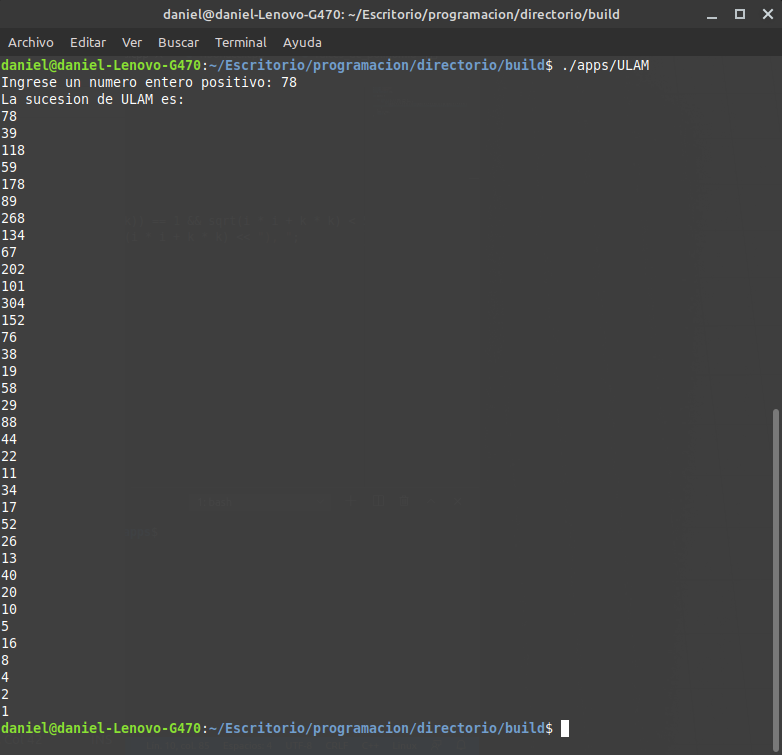
\includegraphics[width=0.8\textwidth]{figures/ULAM}
  \caption{Ejecución de algunas instancias del problema.}
  \label{fig:ULAM}
\end{figure}
\newpage

\section{Ejercicio 11.}

Un tri\'angulo recto puede tener lados cuyas longitudes sean valores enteros. El conjunto de tres valores enteros para las longitudes de los lados de un tri\'angulo recto se conoce como triple de Pit\'agoras. 
Las longitudes de los tres lados deben satisfacer la relaci\'on que establece que la suma de los cuadrados de dos lados es igual al cuadrado de la hipotenusa.
Escriba una aplicaci\'on para encontrar todos los triples de Pit\'agoras, donde el lado 1, lado 2 y la hipotenusa no sean mayores de 500.

\subsection{Problema computacional.}
\textbf{Objetivo:} Imprimir en pantalla ternas que sean triple de p\'itagoras tal que ningun valor no sea mayor de 500.

\textbf{Entrada:} Un n\'umero entero mayor que 0 que delimite la hipotenusa.

\textbf{Salida:} Ternas que son triples de p\'itagoras.

\subsection{Algoritmo.}
Para solucionar el problema computacional, utizamos un doble ciclo \texttt{for}, el primer ciclo delimitado por $354$ ya que esta cerca del valor maximo que deben de tener los cateros del triangulo rectangulo:
$354 \thickapprox \sqrt{\frac{500^2}{2}}  $. El segundo ciclo delimitado por 500 en el cual se va evaluando el condicional \texttt{if} si la suma del cuadrado de los catetos es un n\'umero entero y si es menor que 500. Y de esta manera el programa es de tipo $O(n^2)$ y no $O(n^3)$.


El código fuente está disponible en mi repositorio de git hub. \cite{url:triple_de_pitagoras}

\subsection{Instancia del problema.}
Como prueba de escritorio, se seleccionaron las siguientes instancias del problema. Entrada: 40, 100 y 800. La salida del programa se observa en la Figura \ref{fig:triple_de_pitagoras}.
\begin{figure}[ht!]
  \centering
  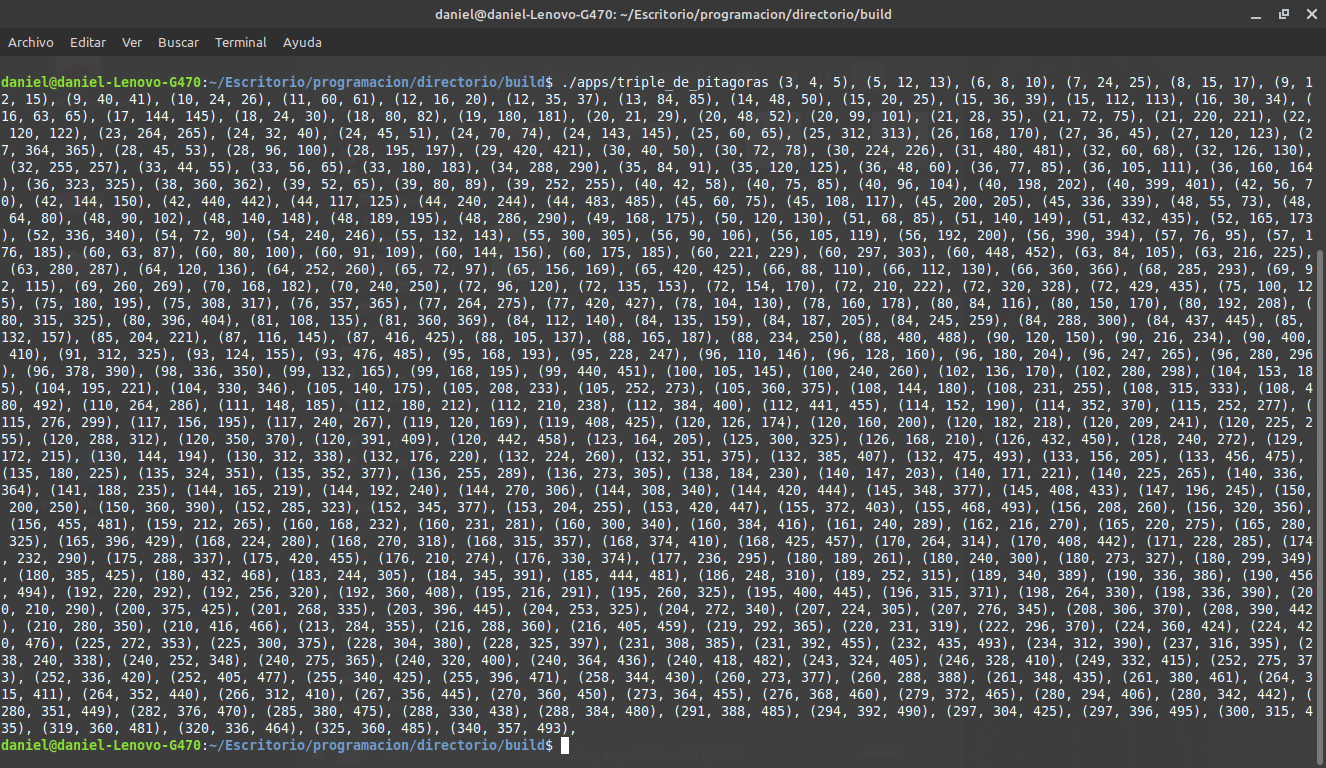
\includegraphics[width=0.8\textwidth]{figures/triple_de_pitagoras}
  \caption{Ejecución de algunas instancias del problema.}
  \label{fig:triple_de_pitagoras}
\end{figure}


\section{Ejercicio 12.}

Escriba un programa capture un n\'umero e imprima un mensaje indicando si es un n\'umero primo.

\subsection{Problema computacional.}
\textbf{Objetivo:} Dado un n\'umero entero mayor que cero, imprimir si es primo o no.

\textbf{Entrada:} Un n\'umero entero mayor que 0.

\textbf{Salida:} La raspuesta de si el n\'umero dado es primo o no.

\subsection{Algoritmo.}
Para solucionar el problema computacional, partimos de la definici\'on de n\'umero primo el cual un n\'umero se denomina primo si solo es divisible por \'el mismo y por $1$. En este caso primero verificamos si es divisible por 2, si no, entonces mediante un ciclo \texttt{for} recorriendo solo n\'umeros impares delimitado por $n/2$ verificamos si $n$ es divisible.


El código fuente está disponible en mi repositorio de git hub. \cite{url:primo}

\subsection{Instancia del problema.}
Como prueba de escritorio, se seleccionaron las siguientes instancias del problema. Entrada: $n=21$, $n=41$, $n=11$ y $n=423412423323$. La salida del programa se observa en la Figura \ref{fig:primo}.
\begin{figure}[ht!]
  \centering
  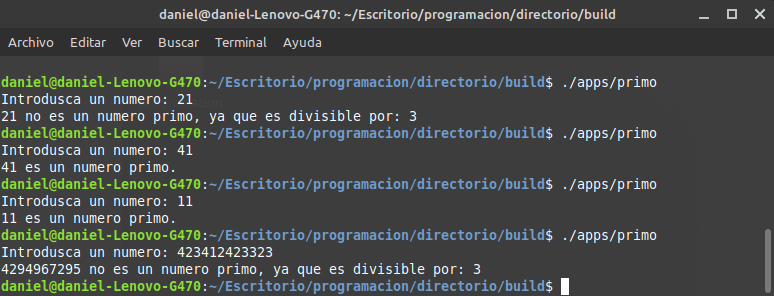
\includegraphics[width=0.8\textwidth]{figures/primo}
  \caption{Ejecución de algunas instancias del problema.}
  \label{fig:primo}
\end{figure}


\section{Ejercicio 13.}

Escriba un programa que capture 15 n\'umeros y los imprima ordenados de menor a mayor.

\subsection{Problema computacional.}
\textbf{Objetivo:} Ordenar una cantidad de $n$ n\'umeros dados por el usuario.

\textbf{Entrada:} Una serie de n\'umeros.

\textbf{Salida:} Los n\'umeros dados por el usuario impresos de menor a mayor.

\subsection{Algoritmo.}
Para solucionar el problema computacional, se utiliz\'o un array para ser m\'as pactico el programa y se aplico un algoritmo de ordenamiento conocido como Selection Sort.


El código fuente está disponible en mi repositorio de git hub. \cite{url:ordenar_numeros}

\subsection{Instancia del problema.}
Como prueba de escritorio, se seleccionó la siguiente instancia del problema. Entrada: 45, 2, 6, 23, 34, 87, 1, 0, 41, 24, 14, 19, 28, 9 y 10 . La salida del programa se observa en la Figura \ref{fig:ordenar_numeros}.
\begin{figure}[ht!]
  \centering
  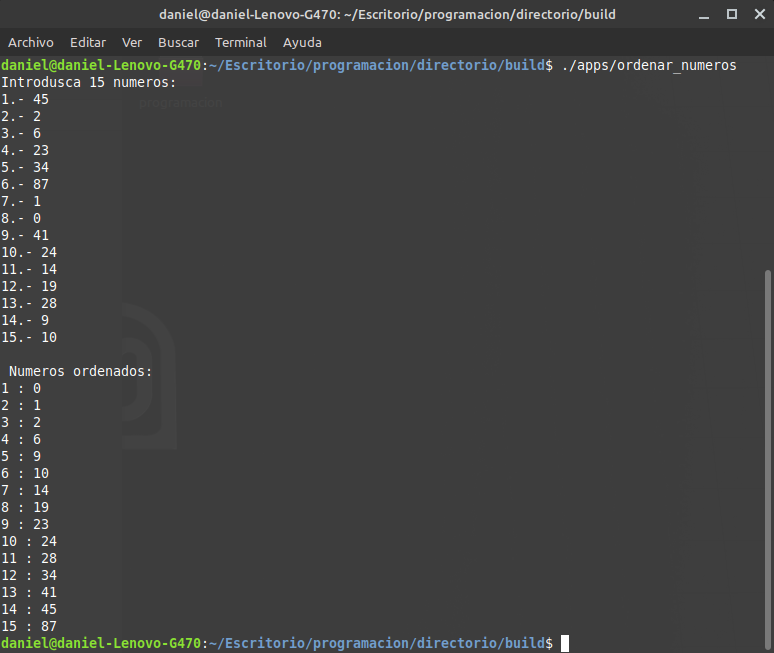
\includegraphics[width=0.8\textwidth]{figures/ordenar_numeros}
  \caption{Ejecución de algunas instancias del problema.}
  \label{fig:ordenar_numeros}
\end{figure}

\newpage



\section{Conclusiones.}
Las Estructura de control condicionada ( \texttt{if-else} o \texttt{switch-case}), estructuras de control por repetici\'on (\texttt{for}, \texttt{while}, \texttt{do-while}) pueden resolver muchos problemas en el cual se requieran ciclos o codiciones, pero si incluimos los array los problemas abarcables son innumerables.

\printbibliography 

\end{document}
